\documentclass[12pt,a4paper]{report}
%
% This LaTeX template has been created by Luca Grilli
% Based on the following https://en.wikibooks.org/wiki/LaTeX/Title_Creation
%
\usepackage[italian]{babel}
\usepackage[T1]{fontenc}
\usepackage{geometry}
\usepackage{graphicx}
\usepackage{hyperref}
\usepackage[utf8]{inputenc}
\usepackage{lipsum} % genera testo fittizio
\usepackage{subcaption}
\usepackage[nottoc,numbib]{tocbibind}
\usepackage{titlesec}

\titleformat{\chapter}[display]{\Huge\bfseries}{}{0pt}{\thechapter.\ }

\graphicspath{{figures/}}
%
%\addtolength{\topmargin}{-.875in} % reduce the default top margin
%\addtolength{\topmargin}{-2cm} % reduce the default top margin
%



%%%%%%%%%%%%%%%%%%%%%%%%%%%%%%%%%%
%                                %
%     Begin Docuemnt [start]     %
%                                %
%%%%%%%%%%%%%%%%%%%%%%%%%%%%%%%%%%
\begin{document}



%%%%%%%%%%%%%%%%%%%%%%%%%%%%%%
%     Title Page [start]     %
%%%%%%%%%%%%%%%%%%%%%%%%%%%%%%
% Declare new goemetry for the title page only.
\newgeometry{margin=1in}
\begin{titlepage}
	\centering
	
\includegraphics[width=0.34\textwidth]{logo-unipg}\par\vspace{1cm}
	\large{Tesina Finale di}\par
	\large{\textbf{Programmazione di Interfacce Grafiche e Dispositivi Mobili}}\par
	\small{Corso di Laurea in Ingegneria Informatica ed Elettronica -- A.A. 2020-2021}\par
	\textsc{\small{Dipartimento di Ingegneria}}\par
	%\large{A.A. 2018-2019}\par

	%\vfill
	\vspace{0.5cm}
	docente\par
	Prof.~Luca \textsc{Grilli}

	\vspace{1cm}
	%\textsc{\large{Tesina Finale a.a. 2018-2019}}\par
	\vspace{1cm}
	\textbf{\huge{JGalaga}}\par
	\vspace{0.2cm}
	applicazione desktop \textsc{JFC/Swing}\par
	%applicazione desktop \textsc{JavaFX}\par
	%app nativa per Android sviluppata con \textsc{AndroidStudio}\par
	\vspace{0.5cm}
	
\includegraphics[width=0.40\textwidth]{circle-cropped-galaga}\par\vspace{1cm}
	\vspace{1cm}

	%\begin{tabular}{ l l l l }
	%\Large{\emph{112233}} & \Large{\emph{Mario}} & \Large{\emph{Rossi}} & \Large{\emph{mario.rossi@studenti.unipg.it}}\\
	%\Large{\emph{114455}} & \Large{\emph{Carlo}} & \Large{\emph{Bianchi}} & \Large{\emph{carlo.bianchi@studenti.unipg.it}}\\
	%\end{tabular}

	\large{studenti}\par
	\vspace{0.2cm}
	\begin{tabular}{ l l l l }
	\large{112233} & \large{\textbf{Mario}} & \large{\textbf{Rossi}} & \large{mario.rossi@studenti.unipg.it}\\
	\large{114455} & \large{\textbf{Carlo}} & \large{\textbf{Bianchi}} & \large{carlo.bianchi@studenti.unipg.it}\\
	\end{tabular}

	%\begin{tabular}{ l l l l }
	%112233 & Mario & Rossi & mario.rossi@studenti.unipg.it\\
	%114455 & Carlo & Bianchi & carlo.bianchi@studenti.unipg.it\\
	%\end{tabular}

	\vfill
	% Bottom of the page
	%{\large \today\par}
	\raggedright
	\small{Data ultimo aggiornamento: \today}
\end{titlepage}
% Ends the declared geometry for the titlepage
\restoregeometry
%%%%%%%%%%%%%%%%%%%%%%%%%%%%
%     Title Page [end]     %
%%%%%%%%%%%%%%%%%%%%%%%%%%%%

%%%%%%%%%%%%%%%%%%%%%%%%%%
%     Indice [start]     %
%%%%%%%%%%%%%%%%%%%%%%%%%%
\tableofcontents
%%%%%%%%%%%%%%%%%%%%%%%%
%     Indice [end]     %
%%%%%%%%%%%%%%%%%%%%%%%%

%%%%%%%%%%%%%%%%%%%%%%%%%%%%%%%%%%%%%%%%%%%%
%     Descrizione del Problema [start]     %
%%%%%%%%%%%%%%%%%%%%%%%%%%%%%%%%%%%%%%%%%%%%
\chapter{Descrizione del Problema}\label{ch:despro}
L'obiettivo di questo lavoro è lo sviluppo di un'applicazione desktop, denominata \emph{JGalaga}, che realizza una versione estremamente semplificata dell'omonimo videogioco arcade~\cite{wiki:it:galaga,wiki:en:galaga}.

L'applicazione sarà implementata utilizzando la tecnologia JFC/Swing in modo da favorire un'ampia portabilità su diversi sistemi operativi (piattaforme), riducendo al minimo eventuali modifiche al codice sorgente. Tuttavia, il codice prodotto sarà testato e ottimizzato per la piattaforma Linux Ubuntu 18.04.

\medskip
Di seguito sarà data una breve descrizione del videogioco originale \emph{Galaga}~\cite{wiki:it:galaga,wiki:en:galaga}, dopodiché si fornirà una descrizione della versione semplificata che si intende realizzare.

%----------------------------------------------
% Sezione: Il Videogioco Arcade Galaga [start]
%----------------------------------------------
\section{Il Videogioco Arcade Galaga}\label{se:gal}
\lipsum[1-2]

\begin{figure}[bt]
\begin{subfigure}{.32\textwidth}
  \centering
  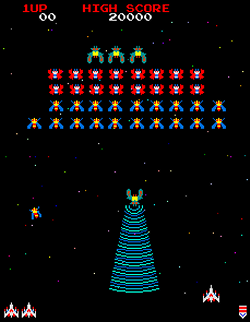
\includegraphics[width=.95\linewidth]{snapshot1}
  %\caption{1a}
  \caption{}
  \label{fig:snap1}
\end{subfigure}%
\begin{subfigure}{.32\textwidth}
  \centering
  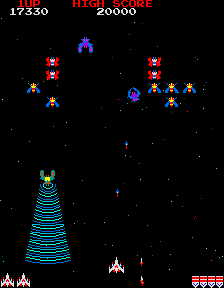
\includegraphics[width=.95\linewidth]{snapshot2}
  %\caption{1a}
  \caption{}
  \label{fig:snap2}
\end{subfigure}%
\begin{subfigure}{.32\textwidth}
  \centering
  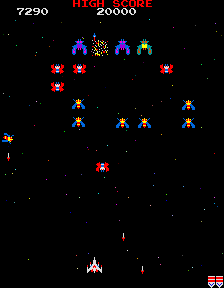
\includegraphics[width=.95\linewidth]{snapshot3}
  %\caption{1b}
  \caption{}
  \label{fig:snap3}
\end{subfigure}
\caption{Tre schermate del videogioco Galaga originale. Le schermate (a) e (b) mostrano una navicella aliena di tipo \emph{boss} che tenta di catturare la navicella del giocatore, emanando il cosiddetto \emph{raggio traente}. La schermata (c) mostra l'esplosione di un navicella aliena.}
\label{fig:fig}
\end{figure}
%----------------------------------------------
% Sezione: Il Videogioco Arcade Galaga [end]
%----------------------------------------------


%----------------------------------------
% Sezione: L'applicazione JGalaga [start]
%----------------------------------------
\section{L'applicazione JGalaga}\label{se:appjgal}
\lipsum[3-8]
%----------------------------------------
% Sezione: L'applicazione JGalaga [end]
%----------------------------------------
%%%%%%%%%%%%%%%%%%%%%%%%%%%%%%%%%%%%%%%%%%
%     Descrizione del Problema [end]     %
%%%%%%%%%%%%%%%%%%%%%%%%%%%%%%%%%%%%%%%%%%



%%%%%%%%%%%%%%%%%%%%%%%%%%%%%%%%%%%%%%%%%%%
%     Specifica dei Requisiti [start]     %
%%%%%%%%%%%%%%%%%%%%%%%%%%%%%%%%%%%%%%%%%%%
%{\let\clearpage\relax \chapter{Specifica dei Requisiti}\label{ch:spereq}}
\chapter{Specifica dei Requisiti}\label{ch:spereq}

L'applicazione JGalaga che si intende realizzare dovrà soddisfare i seguenti requisiti.

\begin{enumerate}
  \item Inserire tre o quattro righe al massimo per descrivere il requisito, adottando uno stile narrativo semplice e diretto come nell'esempio riportato di seguito.
  \item Presenza di un sottofondo musicale attivabile/disattivabile dal pannello di configurazione dell'applicazione.
  \item Presenza di un sottofondo musicale attivabile/disattivabile dal pannello di configurazione dell'applicazione.
  \item Presenza di un sottofondo musicale attivabile/disattivabile dal pannello di configurazione dell'applicazione.
  \item Presenza di un sottofondo musicale attivabile/disattivabile dal pannello di configurazione dell'applicazione.
  \item Presenza di un sottofondo musicale attivabile/disattivabile dal pannello di configurazione dell'applicazione.
  \item Presenza di un sottofondo musicale attivabile/disattivabile dal pannello di configurazione dell'applicazione.
  \item Presenza di un sottofondo musicale attivabile/disattivabile dal pannello di configurazione dell'applicazione.
  \item Presenza di un sottofondo musicale attivabile/disattivabile dal pannello di configurazione dell'applicazione.
  \item Presenza di un sottofondo musicale attivabile/disattivabile dal pannello di configurazione dell'applicazione.
  \item Presenza di un sottofondo musicale attivabile/disattivabile dal pannello di configurazione dell'applicazione.
  \item Presenza di un sottofondo musicale attivabile/disattivabile dal pannello di configurazione dell'applicazione.
  \item Presenza di un sottofondo musicale attivabile/disattivabile dal pannello di configurazione dell'applicazione.
  \item Presenza di un sottofondo musicale attivabile/disattivabile dal pannello di configurazione dell'applicazione.
  \item Presenza di un sottofondo musicale attivabile/disattivabile dal pannello di configurazione dell'applicazione.
  \item Presenza di un sottofondo musicale attivabile/disattivabile dal pannello di configurazione dell'applicazione.
  \item Presenza di un sottofondo musicale attivabile/disattivabile dal pannello di configurazione dell'applicazione.
  \item Presenza di un sottofondo musicale attivabile/disattivabile dal pannello di configurazione dell'applicazione.
  \item Presenza di un sottofondo musicale attivabile/disattivabile dal pannello di configurazione dell'applicazione.
  \item Presenza di un sottofondo musicale attivabile/disattivabile dal pannello di configurazione dell'applicazione.
  \item Presenza di un sottofondo musicale attivabile/disattivabile dal pannello di configurazione dell'applicazione.
\end{enumerate}
%%%%%%%%%%%%%%%%%%%%%%%%%%%%%%%%%%%%%%%%%
%     Specifica dei Requisiti [end]     %
%%%%%%%%%%%%%%%%%%%%%%%%%%%%%%%%%%%%%%%%%



%%%%%%%%%%%%%%%%%%%%%%%%%%%%
%     Progetto [start]     %
%%%%%%%%%%%%%%%%%%%%%%%%%%%%
\chapter{Progetto}\label{ch:prog}
\lipsum[9]

% Architettura del Sistema Software [start]
%-------------------------------------------
\section{Architettura del Sistema Software}\label{ch:arch}
\lipsum[10]

\begin{figure}[bt]
\begin{subfigure}{.49\textwidth}
  \centering
  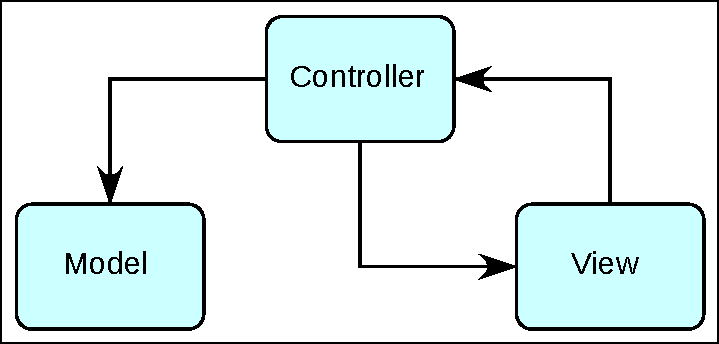
\includegraphics[width=.94\linewidth]{mvc}
  %\caption{1a}
  \caption{}
  \label{fig:mvc}
\end{subfigure}%
\begin{subfigure}{.49\textwidth}
  \centering
  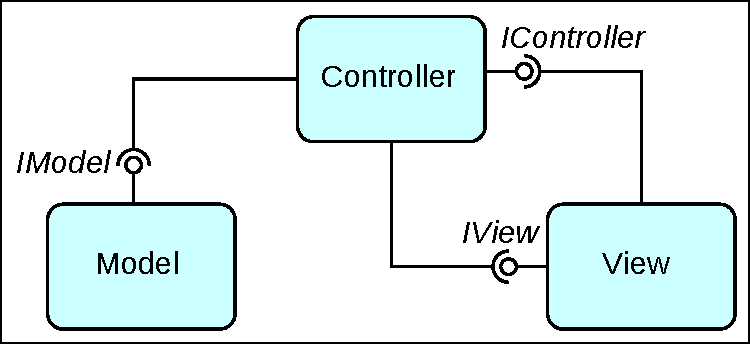
\includegraphics[width=.98\linewidth]{mvc-interfaces}
  %\caption{1a}
  \caption{}
  \label{fig:mvc-int}
\end{subfigure}%
\caption{Architettura  \emph{Model View Controller} (\emph{MVC}) del sistema JGalaga, ove sono evidenziate: (a) le direzioni dei principali flussi informativi, cio\`e quali moduli possono inviare determinati messaggi e quali altri moduli possono riceverli; (b) le interfacce esposte dai singoli moduli architetturali al fine di ridurre l'accoppiamento tra classi di moduli distinti.}
\label{fig:arch}
\end{figure}

\lipsum[10 -11]
% Architettura del Sistema Software [end]
%-------------------------------------------

% Model [start]
%-------------------------------------------
\section{Model}\label{se:arch.model}
\lipsum[12]
In Fig.~\ref{fig:model} viene illustrato il digramma di classe del modulo Model.\newline
\textbf{N.B.} si tratta di un esempio che in realtà non ha nulla a che fare con il videogame JGalaga!

\begin{figure}[tb]
  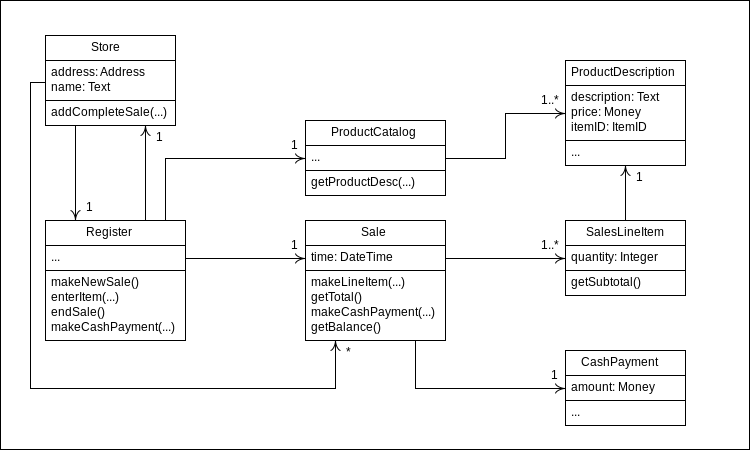
\includegraphics[width=\linewidth]{ModelClassDiagram}
  \caption{Diagramma di classe del modulo Model. Si tratta in realt\`a di un esempio che non ha nulla a che fare con il videogame JGalaga!}
  \label{fig:model}
\end{figure}

\lipsum[13-15]
\medskip

Generalmente un diagramma di classe, come ogni diagramma UML, illustra una vista semplificata di un sistema. Per tale ragione, pu\`o anche essere prodotto con carta e penna, senza avvalersi di editor UML. Anzi, i diagrammi creati manualmente conferiscono al documento un forte carattere di progettualit\`a e creativit\`a. Per tale ragione si stanno diffondendo degli strumenti on-line per produrre diagrammi che sembrano essere creati con carta e penna~\cite{yUML}.

\begin{figure}[tb]
  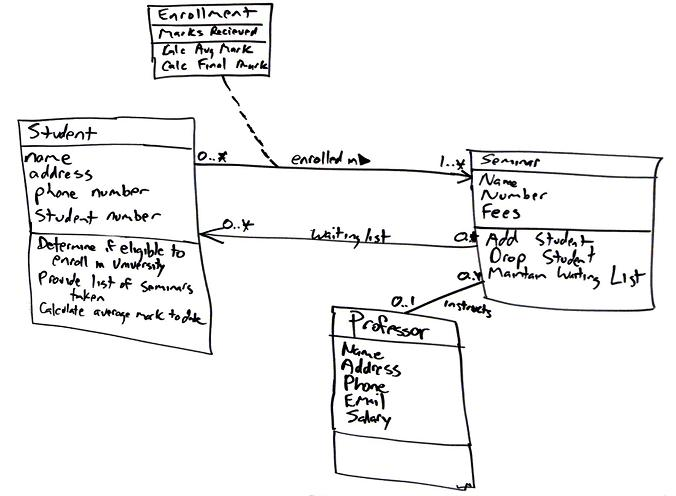
\includegraphics[width=\linewidth]{classDiagramSketch}
  \caption{Diagramma di classe UML di tipo ``sketch''. Si tratta in realt\`a di un esempio che non ha nulla a che fare con il videogame JGalaga!}
  \label{fig:model-sketch}
\end{figure}

\lipsum[14]
% Model [end]
%-------------------------------------------

% View [start]
%-------------------------------------------
\section{View}\label{se:arch.view}
\lipsum[16]

\begin{figure}[tb]
  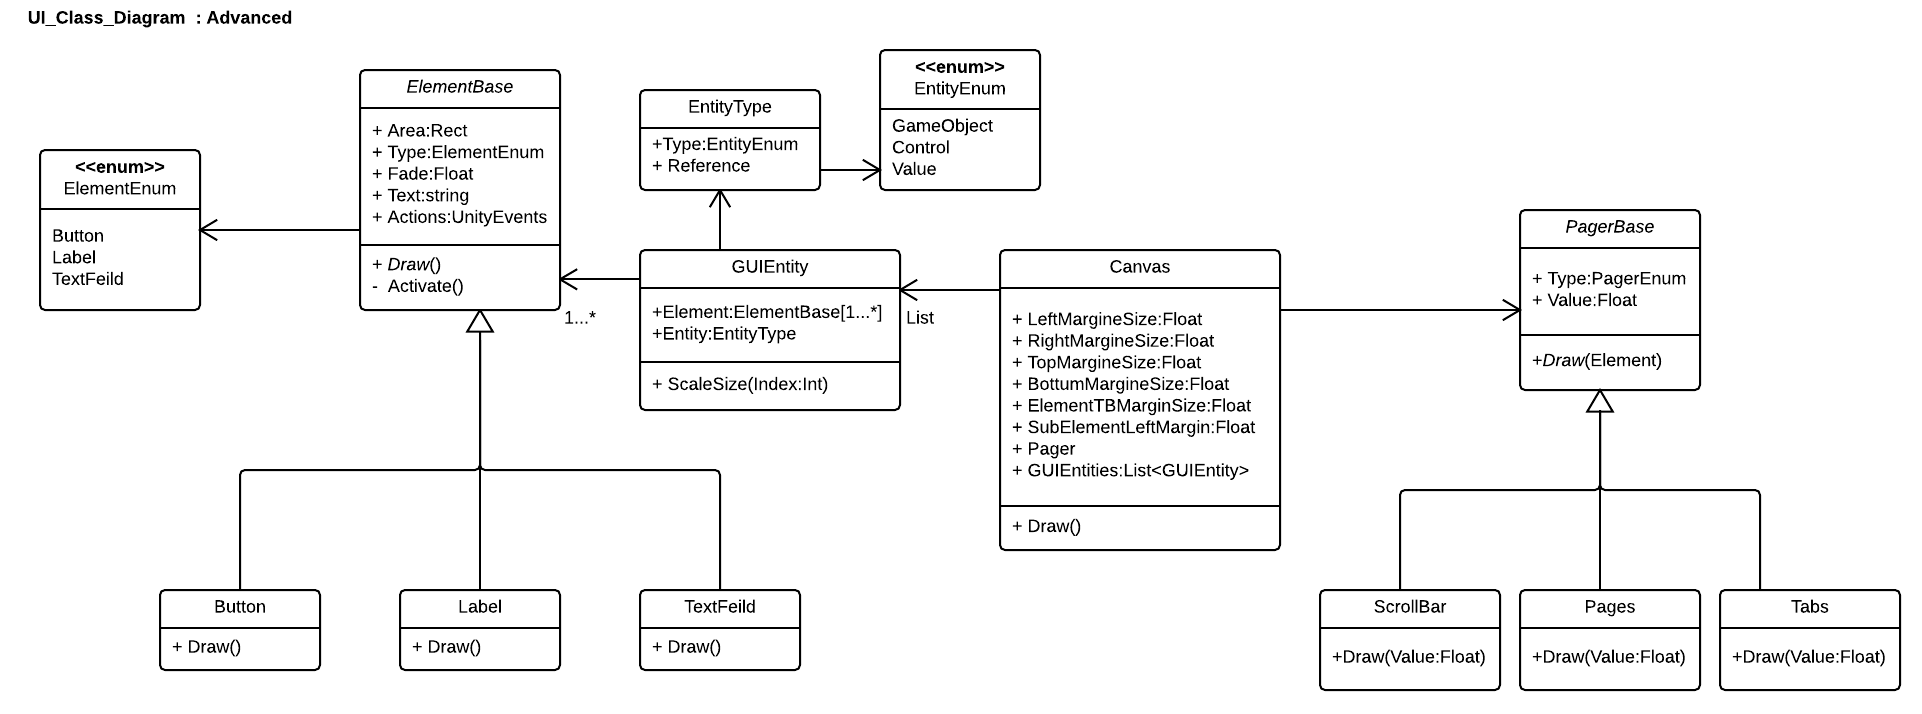
\includegraphics[width=\linewidth]{UI-Class-Diagram-Advanced}
  \caption{Diagramma di classe del modulo View. Si tratta in realt\`a di un esempio che non ha nulla a che fare con il videogame JGalaga!}
  \label{fig:view}
\end{figure}

\lipsum[17-19]
% View [end]
%-------------------------------------------

% Controller [start]
%-------------------------------------------
\section{Controller}\label{se:arch.cont}
\lipsum[20]

\begin{figure}[tb]
  \centering
  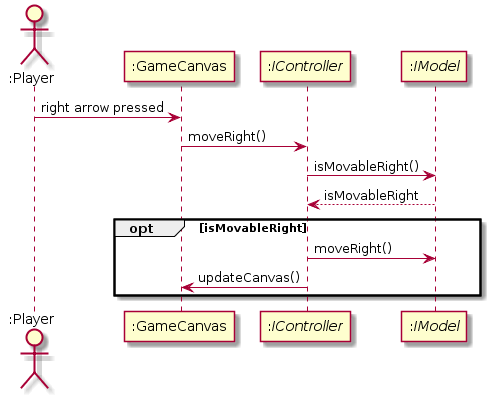
\includegraphics[width=.70\linewidth]{SequenceDiagram-PlantText.png}
  \caption{Diagramma di sequenza che illustra la gestione dell'evento ``spostamento a destra'' della navicella controllata dal giocatore in JGalaga.}
  \label{fig:controller-seq-diag}
\end{figure}

\lipsum[21-22]

\begin{figure}[bt]
  \centering
  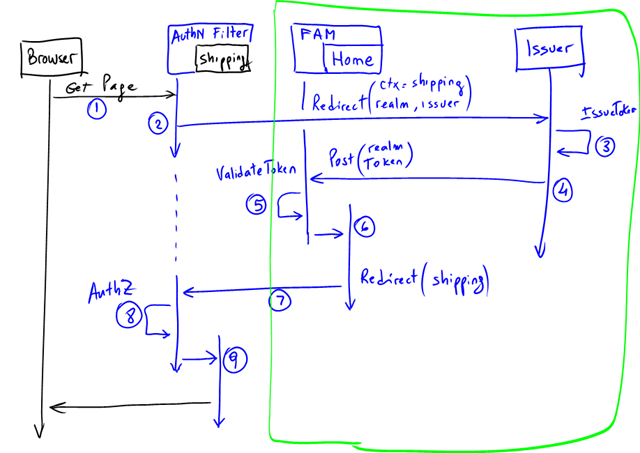
\includegraphics[width=.80\linewidth]{controller-sketched.png}
  \caption{Diagramma di sequenza UML di tipo ``sketch''. Si tratta in realt\`a di un esempio che non ha nulla a che fare con il videogame JGalaga!}
  \label{fig:controller-sketched}
\end{figure}

\lipsum[23-24]
% Controller [end]
%-------------------------------------------

% Problemi Riscontrati [start]
%-------------------------------------------
\section{Problemi Riscontrati}\label{ch:proris}
% Problemi Riscontrati [end]
\lipsum[25]

Si riportano di seguito i principali problemi riscontrati nello svolgimento del progetto JGalala. 
\begin{itemize}
\item Descrizione del primo problema riscontrato ...
\item Descrizione del secondo problema riscontrato ...
\item Descrizione del terzo problema riscontrato ...
\item ...
\item ...
\item ...
\item Descrizione dell'ultimo problema riscontrato ...
\end{itemize}

\lipsum[26-28]
% Problemi Riscontrati [stop]
%-------------------------------------------
%%%%%%%%%%%%%%%%%%%%%%%%%%
%     Progetto [end]     %
%%%%%%%%%%%%%%%%%%%%%%%%%%



%%%%%%%%%%%%%%%%%%%%%%%%%%%%%%%%%%%%%%%%%%%%%%%%%
%     Conclusioni e sviluppi futuri [start]     %
%%%%%%%%%%%%%%%%%%%%%%%%%%%%%%%%%%%%%%%%%%%%%%%%%
\chapter{Conclusioni e sviluppi futuri}\label{ch:conc-svil-fut}
\lipsum[29-30]
%%%%%%%%%%%%%%%%%%%%%%%%%%%%%%%%%%%%%%%%%%%%%%%
%     Conclusioni e sviluppi futuri [end]     %
%%%%%%%%%%%%%%%%%%%%%%%%%%%%%%%%%%%%%%%%%%%%%%%


%%%%%%%%%%%%%%%%%%%%%%%%%%%%%%%%%%%%%%%%%%%%%
%     Bibliografia e Sitografia [start]     %
%                 NO BibTeX                 %
%%%%%%%%%%%%%%%%%%%%%%%%%%%%%%%%%%%%%%%%%%%%%
%\chapter{Bibliografia e Sitografia}\label{ch:bibsit}
%
%\begin{thebibliography}{9}
%\bibitem{lamport94}
%  Leslie Lamport,
%  \textit{\LaTeX: a document preparation system},
%  Addison Wesley, Massachusetts,
%  2nd edition,
%  1994.
%\end{thebibliography}
%
%%%%%%%%%%%%%%%%%%%%%%%%%%%%%%%%%%%%%%%%%%%
%     Bibliografia e Sitografia [end]     %
%                 NO BibTeX               %
%%%%%%%%%%%%%%%%%%%%%%%%%%%%%%%%%%%%%%%%%%%



%%%%%%%%%%%%%%%%%%%%%%%%%%%%%%%%%%%%%%%%%%%%%
%     Bibliografia e Sitografia [start]     %
%                with BibTeX                %
%%%%%%%%%%%%%%%%%%%%%%%%%%%%%%%%%%%%%%%%%%%%%
\bibliographystyle{plain}
\bibliography{bibliografia}
% inserire i riferimenti bibliografici nel file 'bibliografia.bib'
%%%%%%%%%%%%%%%%%%%%%%%%%%%%%%%%%%%%%%%%%%%
%     Bibliografia e Sitografia [end]     %
%                with BibTeX              %
%%%%%%%%%%%%%%%%%%%%%%%%%%%%%%%%%%%%%%%%%%%



%%%%%%%%%%%%%%%%%%%%%%%%%%%%%
%     Appendice [start]     %
%%%%%%%%%%%%%%%%%%%%%%%%%%%%%
\chapter{Appendice}\label{ch:app}
\lipsum[31-32]
%%%%%%%%%%%%%%%%%%%%%%%%%%%
%     Appendice [end]     %
%%%%%%%%%%%%%%%%%%%%%%%%%%%



\end{document}
%%%%%%%%%%%%%%%%%%%%%%%%%%%%%%%%
%                              %
%     Begin Docuemnt [end]     %
%                              %
%%%%%%%%%%%%%%%%%%%%%%%%%%%%%%%%